\section{Studienablauf}

Der Ablauf der Studie kann sich in drei Phasen untergliedern lassen: die Begrüßungsphase, die VR-Phase und die Abschlussphase. Im Folgenden wird der genaue Ablauf einer Durchführung der Studie beschrieben.

\subsubsection{Einleitungsphase}
Zu aller erst grüßten wir die Probanden und stellten ein paar allgemeine Fragen, wie zum Beispiel ob sie jemals an einer Studie an der Universität teilgenommen haben oder ob sie schon einmal eine VR-Brille aufgesetzt haben. Danach baten wir sie die Formulare durchzulesen und zu unterschreiben. Der Proband setzte sich in einen bequemen Stuhl, welcher von ihm nach Belieben verstellt werden kann. Nachdem wir die Teilnehmer darüber informierten, dass es in dieser Studie darum geht sich möglichst zu Entspannen oder gegebenenfalls einzuschlafen, erklärten wir, wie man die Lehne des Stuhls verstellt (damit sie so bequem wie möglich saßen), erläuterten wir wie der Controller funktioniert und welche Mechanismen für die Aufgaben vonnöten sind. Anschließend wurden die Versuchsteilnehmer mit der VR-Brille vertraut gemacht. Das heißt, wie sie die Brille für ihre Bedürfnisse entsprechend einzustellen haben und falls der Proband ein Brillenträger war, was es noch zusätzlich zu beachten gibt.
Des Weiteren wurden die Probanden ebenfalls über die Freiwilligkeit und die Möglichkeit, zu jeder Zeit im Falle von Unannehmlichkeiten, die Studie abzubrechen unterrichtet.

\begin{figure}[H]
	\centering
	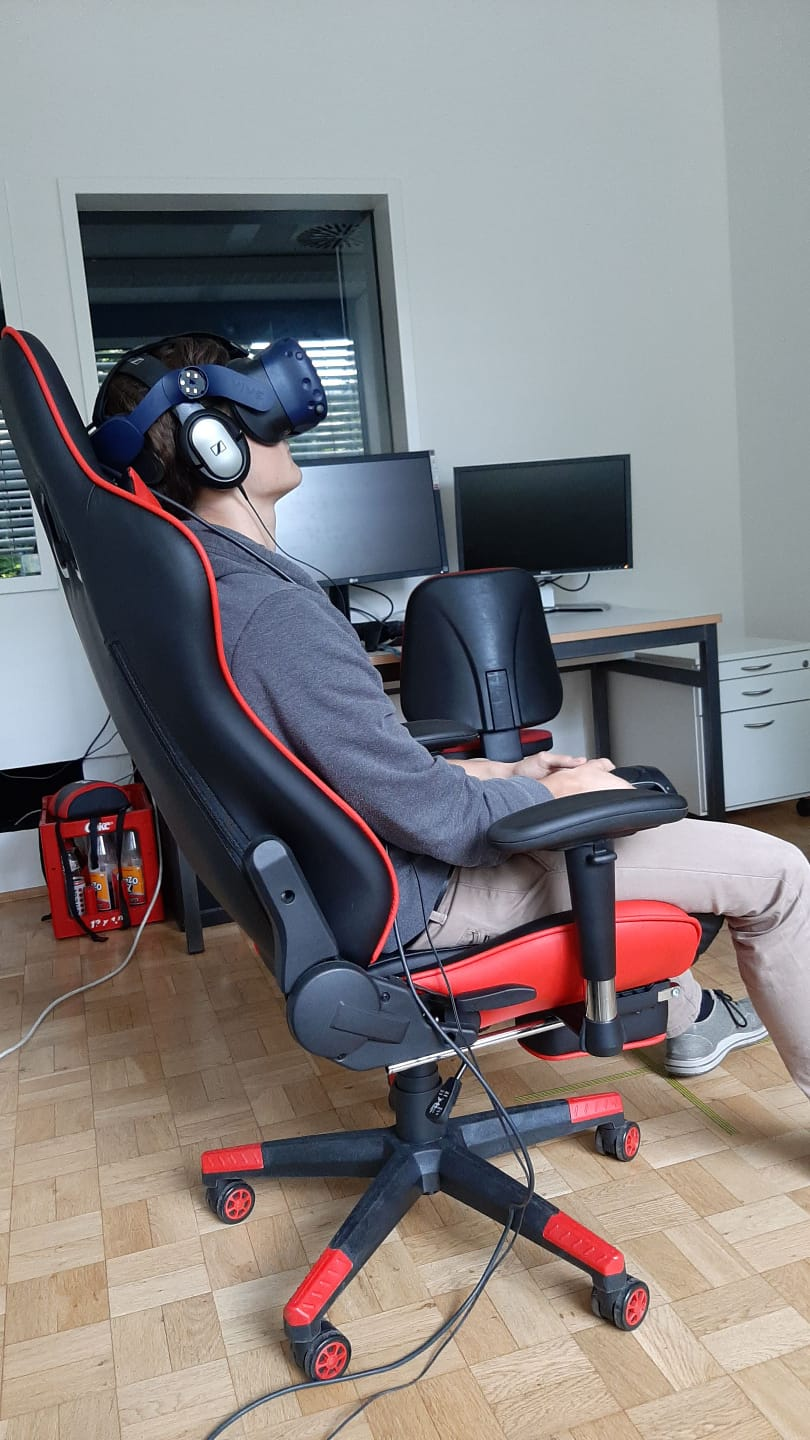
\includegraphics[width=0.6\textwidth]{./images/studie_awf.jpeg}
	\caption{Ein Proband beim Durchführen der Studie.}
	\label{fig:study_setup}
\end{figure}


\subsubsection{VR-Phase}
Nach den einführenden Instruktionen zum Ablauf und zur Bedienung des VR-Controllers, wird dem Proband die VR-Brille aufgesetzt, woraufhin er als erstes einen Begrüßungsscreen sehen konnte, welcher durch einen continue Button weggeklick werden konnte. Dies war der offizielle Start in dem die Zeit gemessen wurde. Nach dem Betätigen des ersten Buttons sah der Teilnehmer einen SAM-Fragebogen, der er ausfüllen musste. In diesem Fragebogen werden einzelne Gemütszustände der Teilnehmer abgefragt, zum einen wie glücklich sie sind und wie aufgeregt und als drittes wie [ \ \ \ ] ... \todoTob{wie kann man das beschreiben? haha}
\todoTob{hier Bild von SAM fragebogen in VR?}

Bevor die eigentliche Studie beginnt, hat der Proband die Möglichkeit, sich ein wenig mit der Steuerung vertraut zu machen, indem er in der Umgebung den Controller verwendet, um schwebende Blasen platzen zu lassen, eine Mechanik die in allen drei späteren Aufgaben von elementarer Bedeutung sein wird. Sobald die Testperson durch das klicken auf einen Button angibt, bereit zu sein, beginnt die Ruhephase. Diese beträgt bei jedem einzelnen Probanden exakt 15 Minuten, jedoch wurde ihnen vor der Studie mitgeteilt, dass die Dauer zwischen 15 und 25 Minuten variiere.

Bei unseren ersten 30 Teilnehmern wurde ein heller Lichtreiz verwendet um die Probanden aus dem Schlaf beziehungsweise aus ihrer Entspannung zu reißen. Bei 15 von ihnen dauerte es 20 Sekunden bis der Lichtreiz seine volle Helligkeit erreichte, wohingegen bei der anderen Hälfte der Lichtreiz fünf Sekunden benötigte um sich vollkommen zu entfalten. Die restlichen 15 Probanden wurden nicht visuell, sondern durch das Geräusch einer Autoalarmanlage geweckt. Jeder Proband wurde innerhalb dieser Phase beobachtet, damit neben Informationen zum Stuhl (Winkel der Lehne) auch festgehalten werden konnte, wie unruhig beziehungsweise entspannt jeder einzelne von ihnen war. Ferner wurde jeder nach zehn Minuten nochmal genauer inspiziert, hierbei wurde die Atmung des Versuchsteilnehmers analysiert.

Bei allen 45 Testpersonen folgte nach dem Wecken die exakt identische Prozedur. Zunächst mussten sie auf einen Startbutton drücken um mit den Aufgaben zu beginnen. Die im Abschnitt 'Aufgaben' geschilderten Tasks wurden stets in derselben Reihenfolge von den Probanden abverlangt. Zuerst das Zahlen sortieren, gefolgt vom Farbspiel und zuletzt das zählen der Blöcke. Hierbei waren die gestellten Aufgaben inhaltelich jedesmal die gleichen. %Noch überlegen, wie wir diese Spiele wirklich nennen wollen.
Sobald der Proband alle drei Aufgaben absolviert hat, muss er abermals den gleichen SAM-Fragebogen wie zuvor ausfüllen und darüber hinaus noch zusätzlich auf die Frage antworten, als wie anspruchsvoll er die gestellten Aufgaben erachtete.\todoTob{hier Bild von sliderfragebogen in VR?} Schlussendlich darf die VR-Brille abgesetzt werden, was dem Teilnehmer durch einen Text in der VR Umgebung mitgeteilt wurde.

\subsubsection{Abschlussphase}
Nachdem der Hauptteil der Studie komplettiert wurde und das VR-Headset abgenommen werden konnte, mussten die Probanden noch eine demographischen Umfrage bearbeiten, welche diesmal nicht in VR stattfand, sondern an einem Computer im selben Raum. Dieser Fragebogen besteht zu Beginn aus allgemeinen, anonymen Fragen zur Person, Alter des Probanden, Geschlecht, gegebenenfalls der Studiengang, sowie ob der Proband schon vor der Studie Erfahrungen mit VR/AR gemacht hat. Anschließend musste der Versuchsteilnehmer Fragen zur Studie ausfüllen. Ob sich der Proband vor beziehungsweise nach der Studie müde gefühlt hat oder auch ob ein permanentes Tragen einer VR/AR-Brille vorstellbar wäre.
Nachdem dieser Fragebogen vollständig ausgefüllt wurde, fragten wir dir Teilnehmer noch wie lange ihnen die Ruhephase, bzw. die eigentliche Schlafphase, vorgekommen ist und notierten dies für Vergleiche. Zusätzlichen waren wir hier noch offen für allgemeine Anmerkungen ehe wir ihnen das Geld überreichten und sie verabschiedeten.
